\documentclass[document.tex]{subfiles}
\begin{document}
\section*{Exercise 1:}

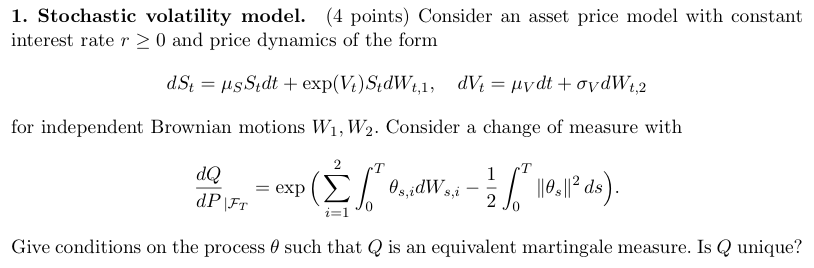
\includegraphics[width=\textwidth]{ex1.png}
Conversely 
\begin{itemize}
	\item $\theta$ must be adapted so $\theta_t$ has to be  $\mathcal{F}_t$ measurable for all $t$ \\ 
	\item $P \lb \frac{dQ}{dP} > 0 \rb =1 $
	\item $1 = E \lb \frac{dQ}{dP} \rb$ 
\end{itemize}

For $Q$ being a equivalent martingale measure the discounted asset price process $\tilde{S} = \frac{S}{S^0}$ with \\ 
Since r is constant $S^0 (t) = exp \lb \int_0^t r_s ds \rb = exp(rt)$  has to be a martingale so $\tilde{S_0}= E^Q_0 \lb \tilde{S} \rb$.\\

applying Ito's product formula to $\tilde{S}$ gives
\begin{align}
	d \tilde{S} = d \frac{S}{S^0}
	= \frac{1}{S^0} d S + S d \frac{1}{S^0}  \label{eq:itoProduct}
  \end{align}
We see that $S^0=e^{rt}$ solves the ODE $d \frac{1}{S^0}=-r \frac{1}{S^0} dt$
therefore we can substitud back into the equation \eqref{eq:itoProduct} and get
\begin{align}
	d \tilde{S} &= e^{-rt} d S - S r e^{-rt} dt \\
	&= e^{-rt} \lb \mu_s S_t dt + e^{V_t} S_t dW_{t,1} \rb  - S r e^{-rt} dt 
\end{align}
applying Girsanov, 2-dimensions $W_{t,1} = \tilde{W}_{t,1} + \int_0^t \theta_{s,1} ds$ and that $\tilde{W}$ is a Brownian Motion under Q.	
\begin{align}
	= e^{-rt} \lb \mu_s S_t dt + e^{V_t} S_t \lb d\tilde{W}_{t,1} + \theta_{d,1} dt \rb \rb  - S r e^{-rt} dt \\
\end{align}

\begin{align}
	-r + \mu_s + e^{V_t} \theta_{t,1} =0 \\
	\theta_{t,1} = \frac{r-\mu_s}{e^{V_t}}
\end{align}
The same reasoning also works for $\tilde{V}$ and $\theta_{t,2}$
\begin{align*}
	d \tilde{V} = e^{-rt} d V_t - V_t r e^{-rt} dt \\
	\dots \\
	\theta_{t,2} = \frac{V_t r - \mu_V }{\sigma_V}
\end{align*}

\end{document}
